\documentclass[12pt, centerh1]{article}
\textwidth=165mm \headheight=0mm \headsep=10mm \topmargin=0mm
\textheight=220mm %\footskip=1.5cm
\oddsidemargin=0mm
%\documentclass[12pt,letterpaper]{article}
%\usepackage[margin=1in]{geometry}
\RequirePackage[colorlinks,citecolor=blue,urlcolor=blue]{hyperref}
\usepackage{amsmath, amssymb,natbib}
%\usepackage[mathscr]{euscript}
%\usepackage{mathrsfs}
\usepackage{graphicx,bm}
\usepackage{color}
\usepackage{subcaption}
 \usepackage[table]{xcolor}
\usepackage{longtable}
\usepackage{amsthm}
\usepackage[mathscr]{euscript}
\usepackage{relsize}
\newcolumntype{P}[1]{>{\centering\arraybackslash}p{#1}}
\usepackage{rotating}
\usepackage{eurosym}
\usepackage{colonequals}
\usepackage{bbm}

\usepackage{listings}


\lstset{language=R}  
\DeclareMathOperator*{\argmax}{argmax}
\DeclareMathOperator*{\argmin}{argmin}

\newcommand{\MM}{\bm{M}}
\newcommand{\MV}{\bm{V}}
\newcommand{\MU}{\bm{U}}
\newcommand\ddfrac[2]{\frac{\displaystyle #1}{\displaystyle #2}}
\newcommand\fancyV{\mathcal{V}}
\newcommand\fancyA{\mathcal{A}}
\newcommand{\tupsi}{\bm{\upsilon}}
\newtheorem{theorem}{Theorem}
 
%\usepackage{titling}
%\usepackage{lipsum}

\newcommand{\bmt}{\bm{\theta}}
\newcommand{\bmx}{\bm{x}}
\newcommand{\bmX}{\bm{X}}
\newcommand{\bmmu}{\bm{\mu}}
\newcommand{\bmSg}{\bm{\Sigma}}

\begin{document}
\section*{Q3}
\subsection*{a)}


Gradient boosting is a technique for optimizing either a regression or classification problem. In our specific case, we look at the classification of diabetes. This differs from the previous method used in that this method is a supervised learning approach. In supervised learning, labels in the training set already known to the model. This differs from clustering where we have no knowledge of the number of groups. Gradient boosting allows to build a model that is an ensemble. In our case, this ensemble is that of classification or decision trees. In formal terms, given a set of data with $n$ observations and $m$ covariates ($\bm{x_i}$) on some set $D = \{ (x_i,y_i) \}$. A tree ensemble uses $K$ additive functions to predict the output of ($y_i$) written as follows 

$$ \hat{y_i}  = \sum_{k=1}^K \lambda f_k(\bm{x}_i), $$ 

where $f_k$ is a decision tree, and $\lambda$ is a shrinkage parameter. Typically when optimizing gradient boosted tree models one devises a Loss function of the following formula 

$$L^{(t)} = \sum_{i=1}^n l(y_i, \hat{y}^{(t-1)}_i + f_k(\bm{x}_i)) + \phi(f_k) $$

Where $\phi(f_k)$ is a penalization term for the complexity of the model \citep[see][for specific implementation]{gradientboost}. The shrinkage parameter is of particular interest. This is the regularization term in a sense. Each model (tree) in the ensemble contributes to the output $\hat{y_i} $ according to $\lambda$. This method is referred to as model averaging and has been found to outperform each standalone model historically. The tuning of $\lambda$ affects the classification performance of the ensemble, and therefore is the one parameter selected to be optimized using the following procedure. 

\paragraph{Stratified Bootstrapping}
Again for this dataset we use same method previously. To tune the shrinkage parameter we split the dataset according to an 80/20 split. I then further balance the training set by performing a stratified bootstrap. This procedure is performed 50 times for each setting of the shrinkage parameter. The shrinkage parameters selected are $0.005,0.01,0.1,0.2,0.5$. The adjusted Rand index (ARI) is again selected as a performance measure. 

\subsection*{c)}
Again since each covariate is of a different magnitude, scaling would be beneficial when training a model. Pointing out again, the concerning single observation of a large number of pregnancies totalling to $17$ for a diabetic individual shows a large $bmi$ measurement of $40$. In general, a $bmi$ of 30 or greater is considered to be overweight.
Further research into the Pima Indian tribes show a rate of miscarriage among the women which explains the large number of pregnancies for this individual. 

Furthermore, I ran the model on a single bootstrap. With 311 trees. Figure 1 shows the variable importance plot for the model. We see that the $glu$ variable measuring glucose is the obvious factor in determining whether you have diabetes or not. This makes sense that the model would pick up this variable as the single most important one. 

\begin{figure}[!htb]
\caption{Variable importance plot showing which variables have the most influence on prediction.}
\centering
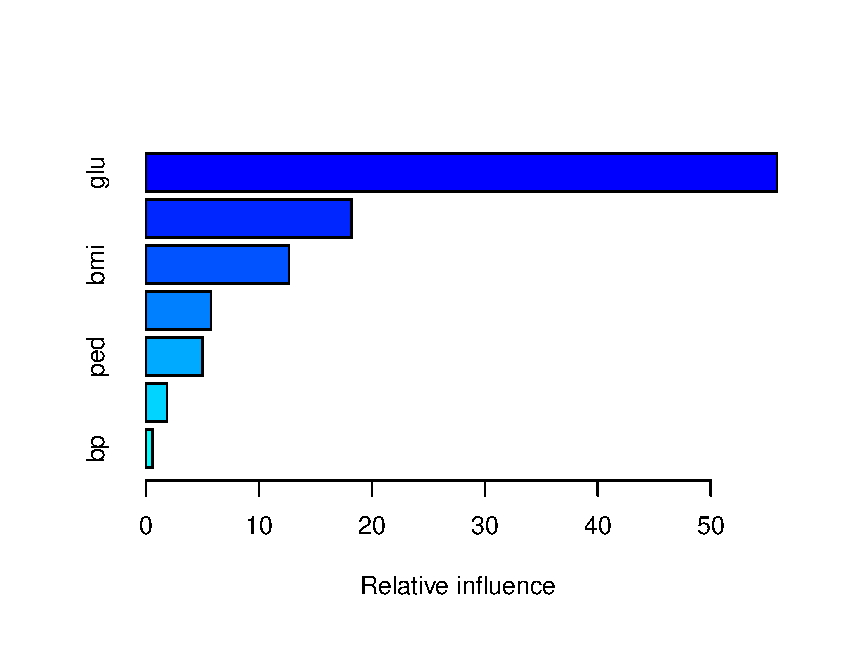
\includegraphics[scale=0.8]{relative_influence}
\end{figure}

After performing a stratified bootstrap on all the settings for the shrinkage parameter, Figure 2 illustrates the ARI for each run. We see that the best ARI on average is for the $\lambda = 0.01$. We also note that the gradient boosted trees model has better ARI performance when compared to the Infinite Gaussian Mixture Model. Note that this is because the boosted trees are a supervised learning method, meaning that we give the labels up front. This shows how powerful supervised learning methods can be. 

\begin{figure}[!htb]
\caption{Variable importance plot showing which variables have the most influence on prediction.}
\centering
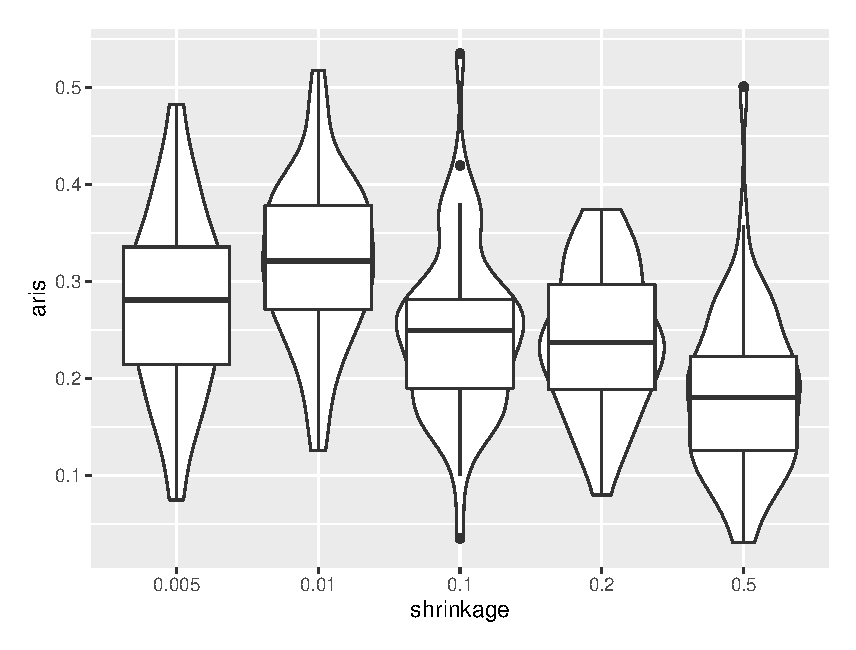
\includegraphics[scale=0.8]{compare_shrinkage}
\end{figure}


\subsection*{d)}
This analysis demonstrates two important findings. The first is that the model can show variable importance. Specifically, the glucose measurement is the single most important parameter to determine diabetes. In contrast, this is a very expensive measurement because it not only has a monetary cost associated with it, but a physical one as well. People do not necessary like getting their blood sampled so I can't imagine scaling this to a large cohort.The second finding is that the shrinkage parameter is very important when determine predictive power. We saw how in Figure 2 that varying it, has an effect on predictive outcome. 


\section*{Q4}

\subsection*{Discussion}
The two methods completely differ in their approaches. The Infinite Gaussian Mixture Model is an unsupervised method that does not even specify the number of groups. As a result it is not as efficient at prediction. We see the ARI is between 0-0.4 which is fairly low. The most interest result of this approach is that it finds multiple clusters that we do not normally consider. There is a sort of ``multiple states" of diabetic ailments; pre-diabetic in a sense. Hence we have those clusters discussed in Q2. In contrast, the gradient boosted trees model (GBM) is a supervised method. We give the labels up front and the model is trained on those specific labels. The issue with this model is it can over-fit. Hence we use a shrinkage parameter to do model averaging. This reduces the problem over-fitting but the parameter must be tuned. By writing my own stratified bootstrap, we balanced the classes and saw across $50$ different bootstraps we have could gain a measure of ARI. Comparing the two methods, the GBM model outperforms the Infinite Gaussian Mixture Model. This is not too surprising since it is indeed a supervised method. 


\end{document}